\documentclass[tikz,border=8pt]{standalone}
\usepackage{amsmath}
\usepackage{pgfplots}
\pgfplotsset{compat=1.18}
\definecolor{ink}{HTML}{21352F}
\definecolor{teal}{HTML}{087F7B}
\definecolor{blue}{HTML}{4B77A8}
\definecolor{gold}{HTML}{C58B2A}
\begin{document}
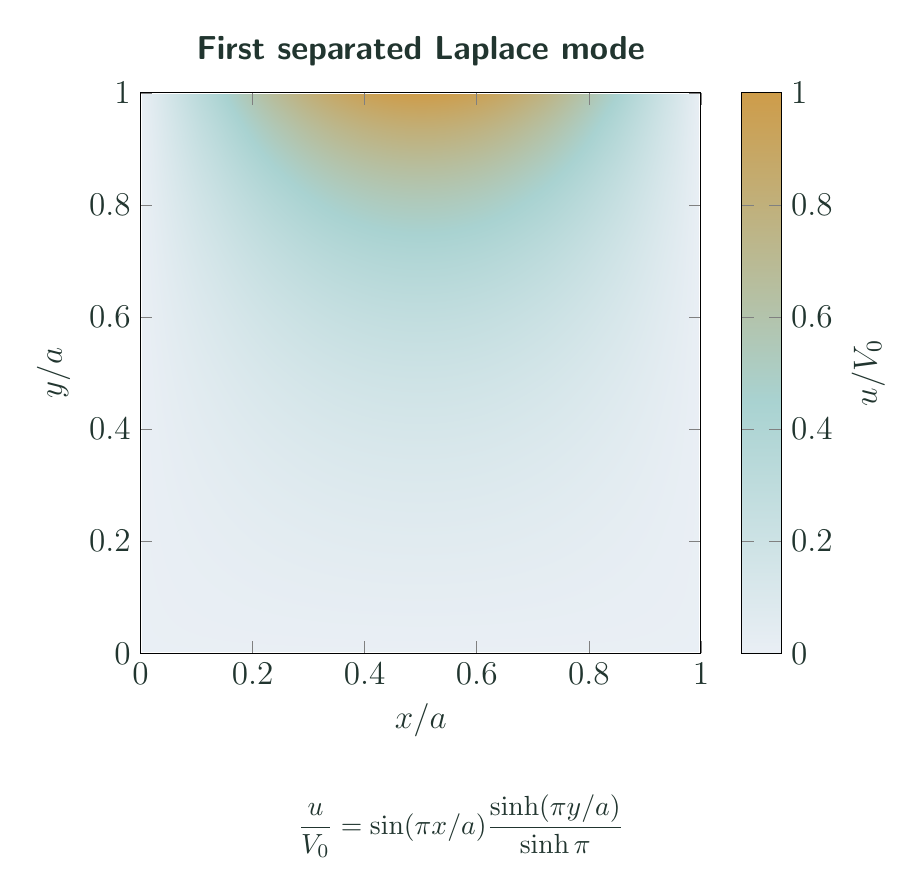
\begin{tikzpicture}[font=\large\sffamily,text=ink]
  \begin{axis}[
    width=11.3cm,height=8.7cm,
    view={0}{90},
    xmin=0,xmax=1,ymin=0,ymax=1,
    xlabel={$x/a$},ylabel={$y/a$},
    axis equal image,
    title={\bfseries First separated Laplace mode},
    colorbar,
    colorbar style={ylabel={$u/V_0$}},
    colormap={academic}{
      color(0cm)=(blue!12);
      color(.45cm)=(teal!35);
      color(1cm)=(gold!85)
    }
  ]
    \addplot3[
      surf,shader=interp,
      domain=0:1,y domain=0:1,
      samples=47,samples y=47,
      point meta=z
    ] {sin(deg(pi*x))*sinh(pi*y)/sinh(pi)};
    \draw[white,very thick] (axis cs:0,0)--(axis cs:1,0)
      --(axis cs:1,1)--(axis cs:0,1)--cycle;
  \end{axis}
  \node[font=\normalsize,below=5mm] at (current bounding box.south)
    {$\displaystyle \frac{u}{V_0}
      =\sin(\pi x/a)\frac{\sinh(\pi y/a)}{\sinh\pi}$};
\end{tikzpicture}
\end{document}
